% !TeX spellcheck = en_US
\addscenariosection{1}{Cooperative Scenario}{Titans' Stronghold}{\images/earthquake.png}

\begin{multicols*}{2}

\textbf{Author:} Invoceusse

\textbf{Source:} \href{https://discord.com/channels/740870068178649108/1219333721019256943}{Archon Studio Discord}

\textit{A long time ago, a mighty fortress was built to house the fantastic and murderous Titans.
  No one has ever entered and returned to tell the tale.
  Now, there are rumors about the death of the guardians and an incredible amount of treasures, potentially including the best bow in the world.\\
  If this legend of the empty fort is true, it's time for excavation.\\
  But for now, you and your allies need to find the keys spread across Antagarich to open the gate of the Titans' Stronghold.
}

\subsection*{\MakeUppercase{Scenario Length}}

This Scenario is played over 16 Rounds (15 on Impossible difficulty).

\subsection*{\MakeUppercase{Player Setup}}

\textbf{Player Count:} 1 -- 6

\textbf{Starting Resources:} 30 \svg{gold}, 8 \svg{building_materials}, 2 \svg{valuables}

\textbf{Starting Income:} 10 \svg{gold}, 2 \svg{building_materials}, 1 \svg{valuables}

\textbf{Starting Units:}
\begin{itemize}
  \item A Pack of \svgunit{bronze} Units of your choice
  \item A Few \svgunit{bronze} Units of your choice
\end{itemize}

\textbf{Town Buildings:} None

\textbf{Map Tile Pool:} None

\textbf{Additional Bonus:} None

\vspace*{\fill}\columnbreak

\subsection*{\MakeUppercase{Map Setup}}

Take the following Map Tiles and arrange them as shown in the Scenario map layout ($P$ stands for the number of players):

\begin{itemize}
  \item P × Starting (I) Map Tile
  \item 2P × Far (II--III) Map Tile
  \item 2P × Near (IV--V) Map Tile
  \item (P + 1) × Center (VI--VII) Map Tile
\end{itemize}

\textbf{\MakeUppercase{Note:}} If you don’t have enough VI--VII Tiles, you can
use another Tile near I Tiles. The center of this
Tile is the Titans’ Stronghold.

\subsection*{\MakeUppercase{Victory Conditions}}

Kill all Units in the Titans' Stronghold (the center of Tile VI--VII next to Tiles I).

\subsection*{\MakeUppercase{Defeat Conditions}}

There are undefeated Units left in the Titans' Stronghold at the end of Round 16 (15 on Impossible difficulty).

\subsection*{\MakeUppercase{Timed Events}}

\textbf{\nth{4}, \nth{8} and \nth{12} Rounds:}
\begin{itemize}
  \item Remove all Black Cubes from every Windmill, Water Wheel, and Mystical Garden on the map.
\end{itemize}

\vspace*{\fill}\columnbreak

\subsection*{\MakeUppercase{Additional Rules}}
\begin{itemize}
  \item Remember: the center of VI--VII Tile next to all I Tiles is the Titans' Stronghold.
  \item No one can enter the Titans' Stronghold until all other VII Fields are flagged by any player.

  \item After defeating a Level VII Neutral army, instead of resolving the Field, the player chooses an option three times from the following list (an option may be chosen multiple times):
    \begin{itemize}
      \item Another player (your choice) gains 5\,\svg{gold}
      \item Another player (your choice) gains 2\,\svg{building_materials}
      \item Another player (your choice) gains 1\,\svg{valuables}
    \end{itemize}
  Then, flag the VII Field with a Faction Cube.
  (There is no bonus in solo play!)

  \item Ignore all yellow borders on Starting Tiles I.
  \item You can use your build Token to give your resources to another player.
  \item Two players can use their build Tokens to exchange Artifacts and/or Spells.

  \item Whenever a player Visits an Obelisk, that player rolls one treasure Die and one resource Die, and resolves one of them.
  \item When all VII Fields (excluding the Titans' Stronghold) are flagged, randomly draw and shuffle the specified number (see the next page) of Neutral Unit Cards from each of their corresponding Decks to create a separate Deck of Neutral Units for the Titans' Stronghold (the Deck of the Titans' Stronghold is sometimes split in two because certain Scenarios are otherwise impossible to implement with the Cards from certain expansions).

  \item Any time a Hero enters the Titans' Stronghold, they draw 5 Cards from the Titans' Stronghold Deck instead of from the Neutral Unit Card Decks. The Units are placed on the Combat Board (see page 29, ``Neutral Unit Setup'' in the Core Rulebook). Players attempt to defeat the Units they find in the Titans' Stronghold. Any Neutral Units defeated during Combat in the Titans' Stronghold are returned to their respective Neutral Unit Decks instead of the Titans' Stronghold Deck. Any Neutral Units surviving Combat in the Titans' Stronghold are shuffled back into the Titans' Stronghold Deck. If there are not enough Unit Cards in this Deck, draw as many Unit Cards as are available and place them on the Combat Board.
  \item Combat in the Titans' Stronghold now costs 1 MP to extend per Combat Round, just like Combat against non-Azure tier Units.
  \item Additionally, no player can:
  \begin{itemize}
    \item Attack other Heroes.
    \item Capture a Mine or Settlement that is already controlled.
  \end{itemize}
\end{itemize}

\vspace*{\fill}

\begin{center}
  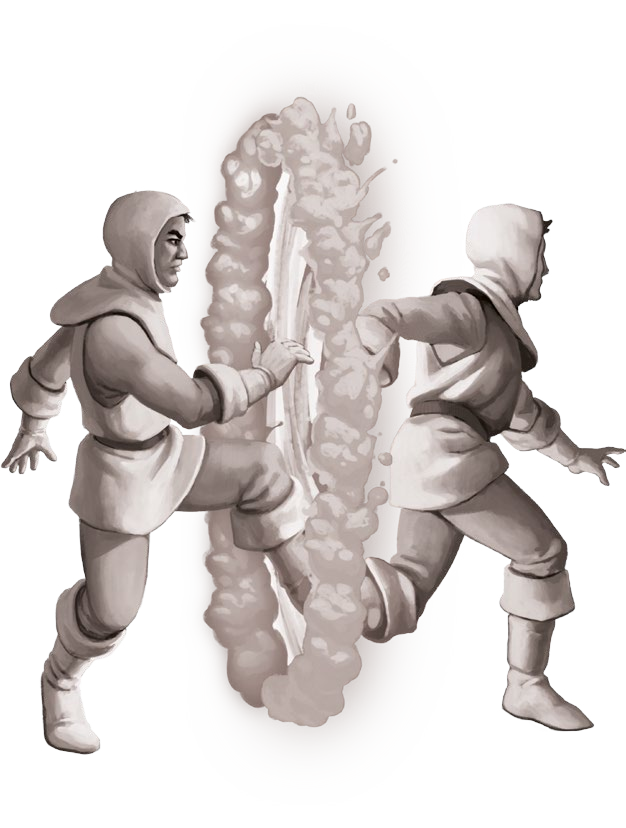
\includegraphics[width=\linewidth]{\art/dimension_door.png}
\end{center}

\vspace*{\fill}

\end{multicols*}

\newpage

\hommtable[]{28}{
  \centering
  \medskip
  \textbf{Strength of Titans' Stronghold Armies}\\
  \bigskip

  \newcommand{\bronze}[0]{\svg[12]{bronze}}
  \newcommand{\silver}[0]{\svg[12]{silver}}
  \newcommand{\golden}[0]{\svg[12]{golden}}
  \newcommand{\azure}[0]{\svg[12]{azure}}

  \begin{tabularx}{\linewidth}{p{0.15\linewidth}XXXX} & \darkcell{Easy} & \darkcell{Normal} & \darkcell{Hard} & \darkcell{Impossible}\\
  \darkcell[1.2]{1 player}
    & \lightcell[1.2]{3\bronze 2\silver 1\golden 1\azure}
    & \lightcell[1.2]{2\bronze 2\silver 2\golden 1\azure}
    & \lightcell[1.2]{2\bronze 2\silver 2\golden 2\azure}
    & \lightcell[1.2]{1\bronze 2\silver 2\golden 3\azure}\\
  \darkcell[1.2]{2 players}
    & \lightcell[1.2]{5\bronze 5\silver 3\golden 1\azure}
    & \lightcell[1.2]{4\bronze 5\silver 3\golden 2\azure}
    & \lightcell[1.2]{2\bronze 5\silver 5\golden 3\azure}
    & \lightcell[1.2]{1\bronze 5\silver 7\golden 4\azure}\\
  \darkcell[1.8]{3 players}
    & \lightcell[1.8]{8\bronze 7\silver 4\golden 2\azure}
    & \lightcell[1.8]{6\bronze 7\silver 5\golden 3\azure}
    & \lightcell[1.8]{2\bronze 3\silver 4\golden 3\azure \linebreak
      Then\linebreak
      2\bronze 4\silver 3\golden 2\azure}
    & \lightcell[1.8]{1\bronze 3\silver 5\golden 3\azure \linebreak
      Then\linebreak
      1\bronze 4\silver 5\golden 3\azure}\\
  \darkcell[1.8]{4 players}
    & \lightcell[1.8]{10\bronze 10\silver 6\golden 2\azure}
    & \lightcell[1.8]{8\bronze 10\silver 6\golden 4\azure}
    & \lightcell[1.8]{2\bronze 5\silver 5\golden 3\azure \linebreak
      Then\linebreak
      2\bronze 5\silver 5\golden 3\azure}
    & \lightcell[1.8]{1\bronze 5\silver 7\golden 4\azure \linebreak
      Then\linebreak
      1\bronze 5\silver 7\golden 4\azure}\\
  \darkcell[1.8]{5 players}
    & \lightcell[1.8]{6\bronze 6\silver 4\golden 1\azure \linebreak
      Then\linebreak
      7\bronze 6\silver 3\golden 2\azure}
    & \lightcell[1.8]{5\bronze 6\silver 4\golden 2\azure \linebreak
      Then\linebreak
      5\bronze 6\silver 4\golden 3\azure}
    & \lightcell[1.8]{3\bronze 6\silver 6\golden 4\azure \linebreak
      Then\linebreak
      3\bronze 6\silver 6\golden 4\azure}
    & \lightcell[1.8]{1\bronze 6\silver 8\golden 6\azure \linebreak
      Then\linebreak
      2\bronze 6\silver 8\golden 5\azure}\\
  \darkcell[1.7]{6 players}
    & \lightcell[1.8]{8\bronze 8\silver 4\golden 1\azure \linebreak
      Then\linebreak
      7\bronze 7\silver 5\golden 2\azure}
    & \lightcell[1.8]{6\bronze 8\silver 4\golden 3\azure \linebreak
      Then\linebreak
      6\bronze 7\silver 5\golden 3\azure}
    & \lightcell[1.8]{3\bronze 8\silver 7\golden 5\azure \linebreak
      Then\linebreak
    3\bronze 7\silver 8\golden 4\azure}
    & \lightcell[1.8]{3\bronze 7\silver 11\golden 6\azure \linebreak
    Then\linebreak
    3\bronze 8\silver 10\golden 6\azure}\\
  \end{tabularx}
}

\vspace*{\fill}

\begin{center}
  \transparent{0.3}{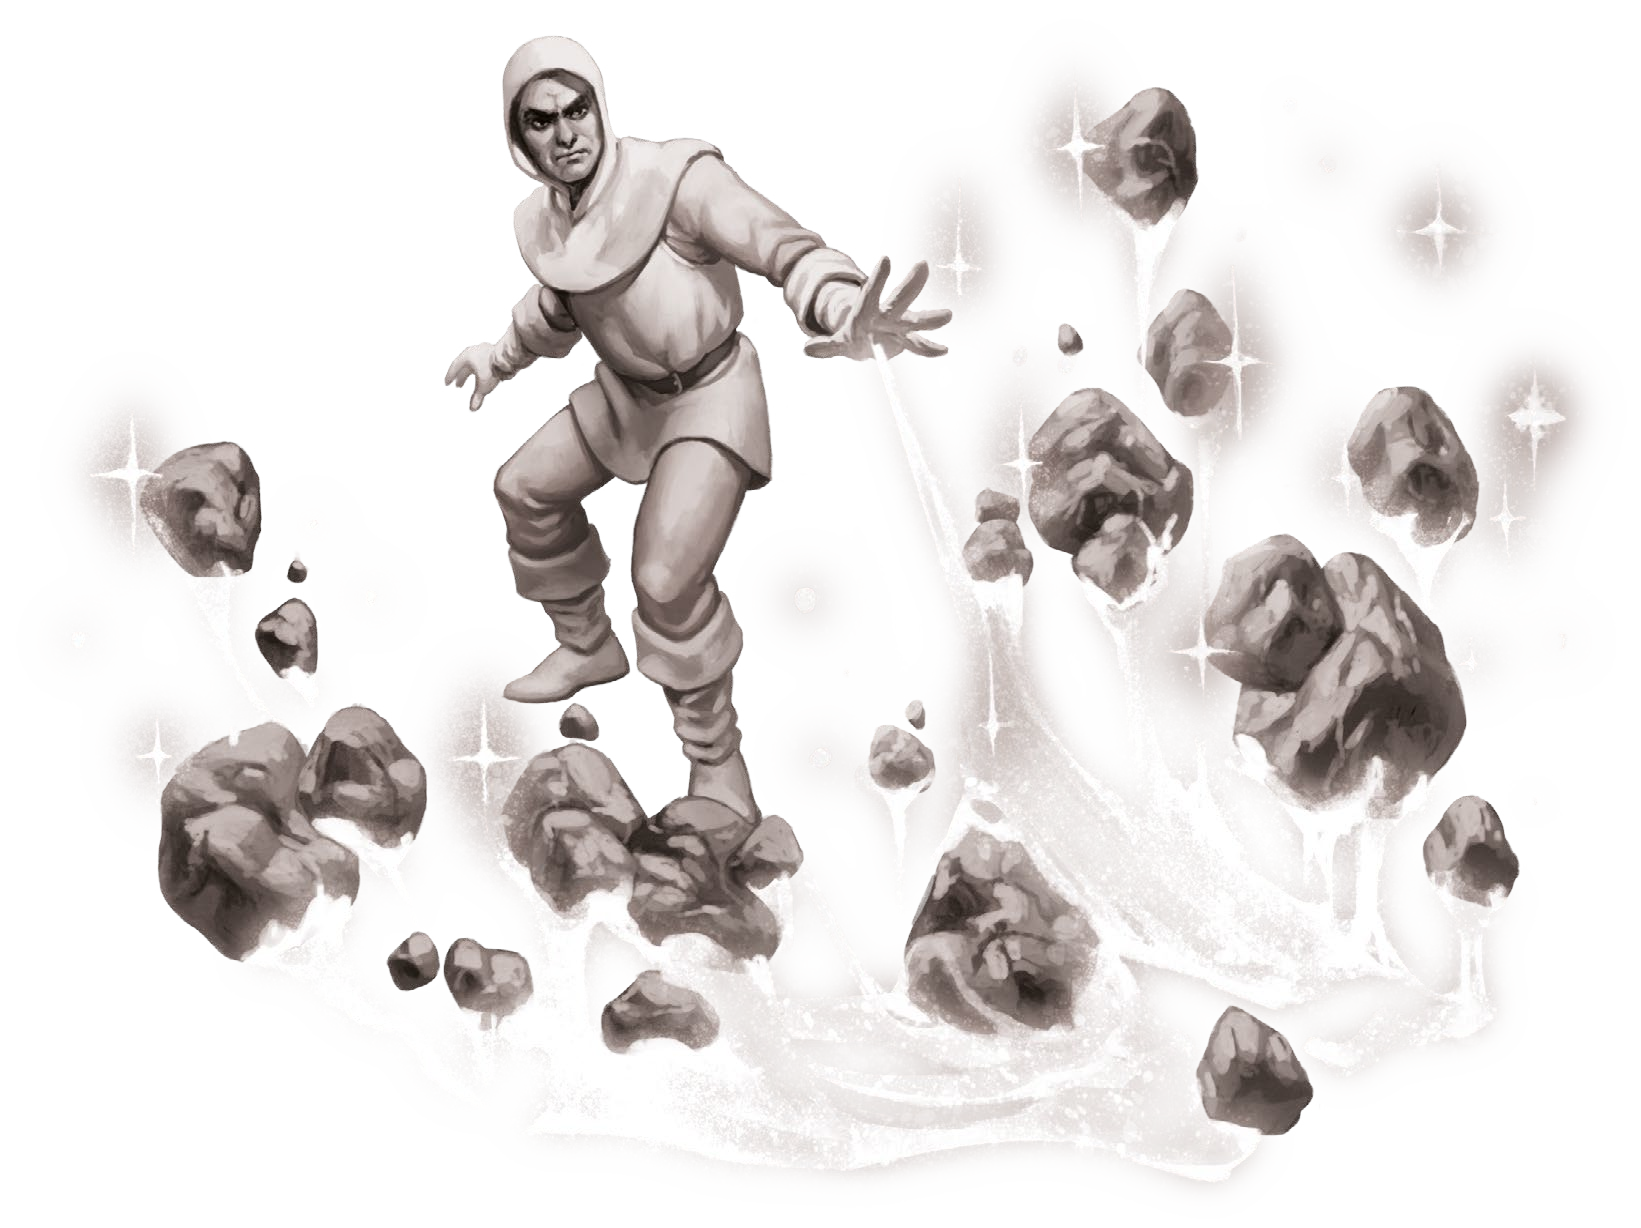
\includegraphics[width=0.6\linewidth, keepaspectratio]{\art/land_mine.png}}
\end{center}

\vspace*{\fill}

\newpage

\begin{minipage}{0.4\paperwidth}
  \centering
  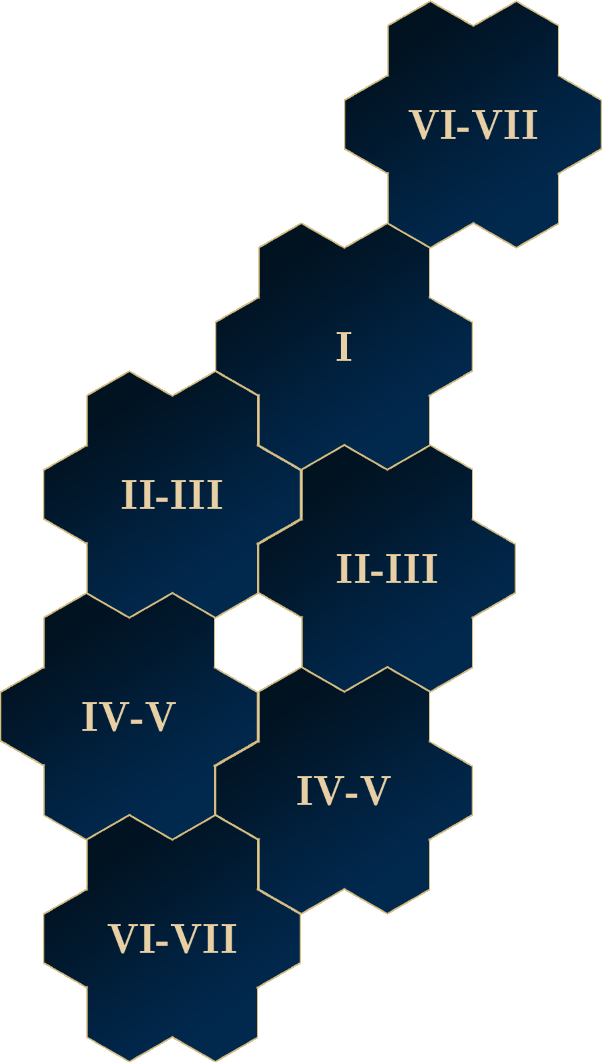
\includegraphics[width=0.18\paperwidth]{\maps/titans-1.png}
  \captionof{figure}{\textbf{1-PLAYER SCENARIO}}
\end{minipage}
\begin{minipage}{0.4\paperwidth}
  \centering
  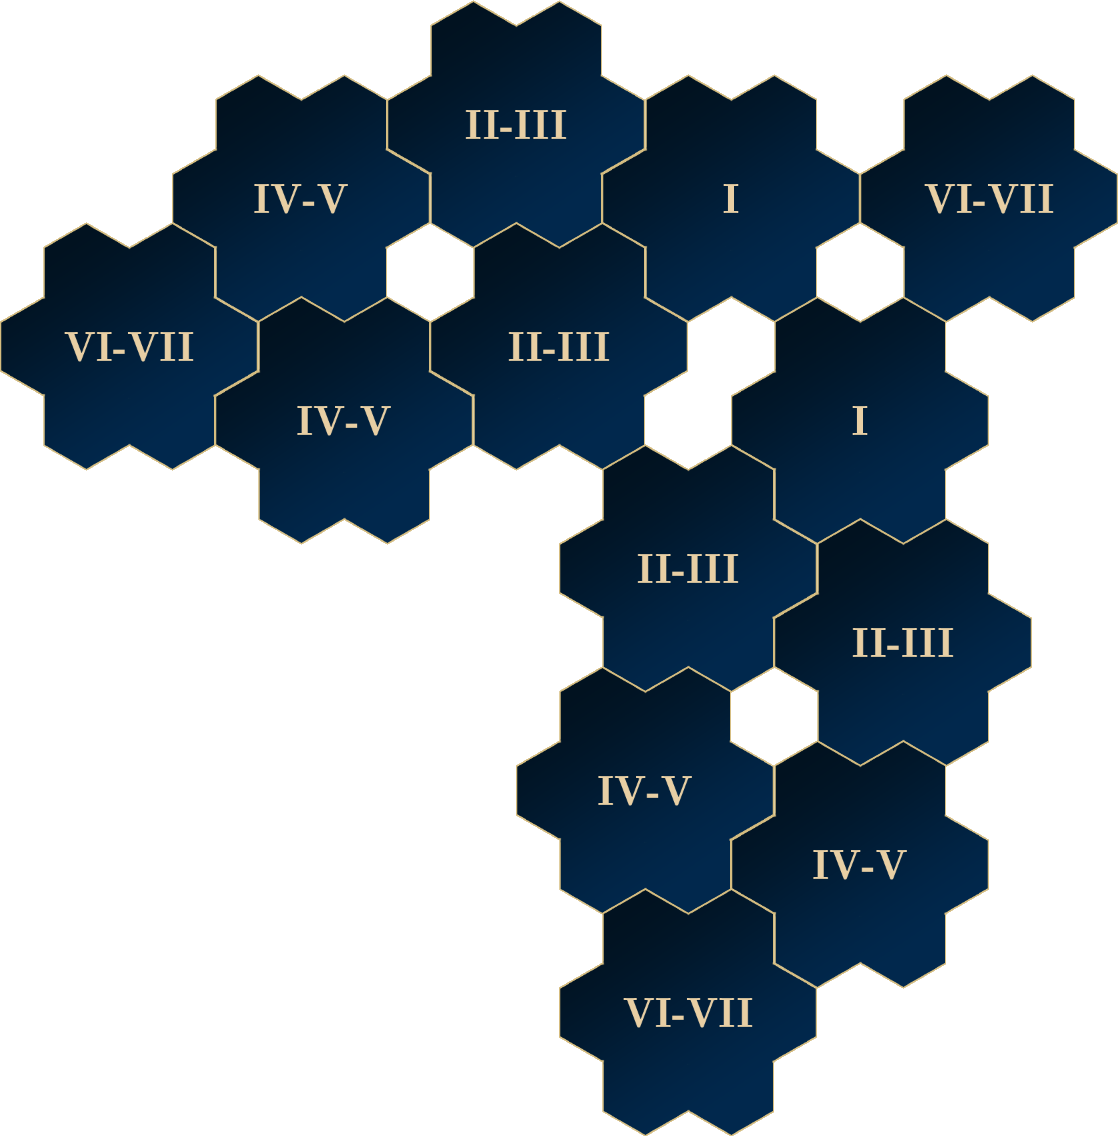
\includegraphics[width=0.36\paperwidth]{\maps/titans-2.png}
  \captionof{figure}{\textbf{2-PLAYER SCENARIO}}
\end{minipage}
\vspace{1em}
\linebreak
\begin{minipage}{0.4\paperwidth}
  \centering
  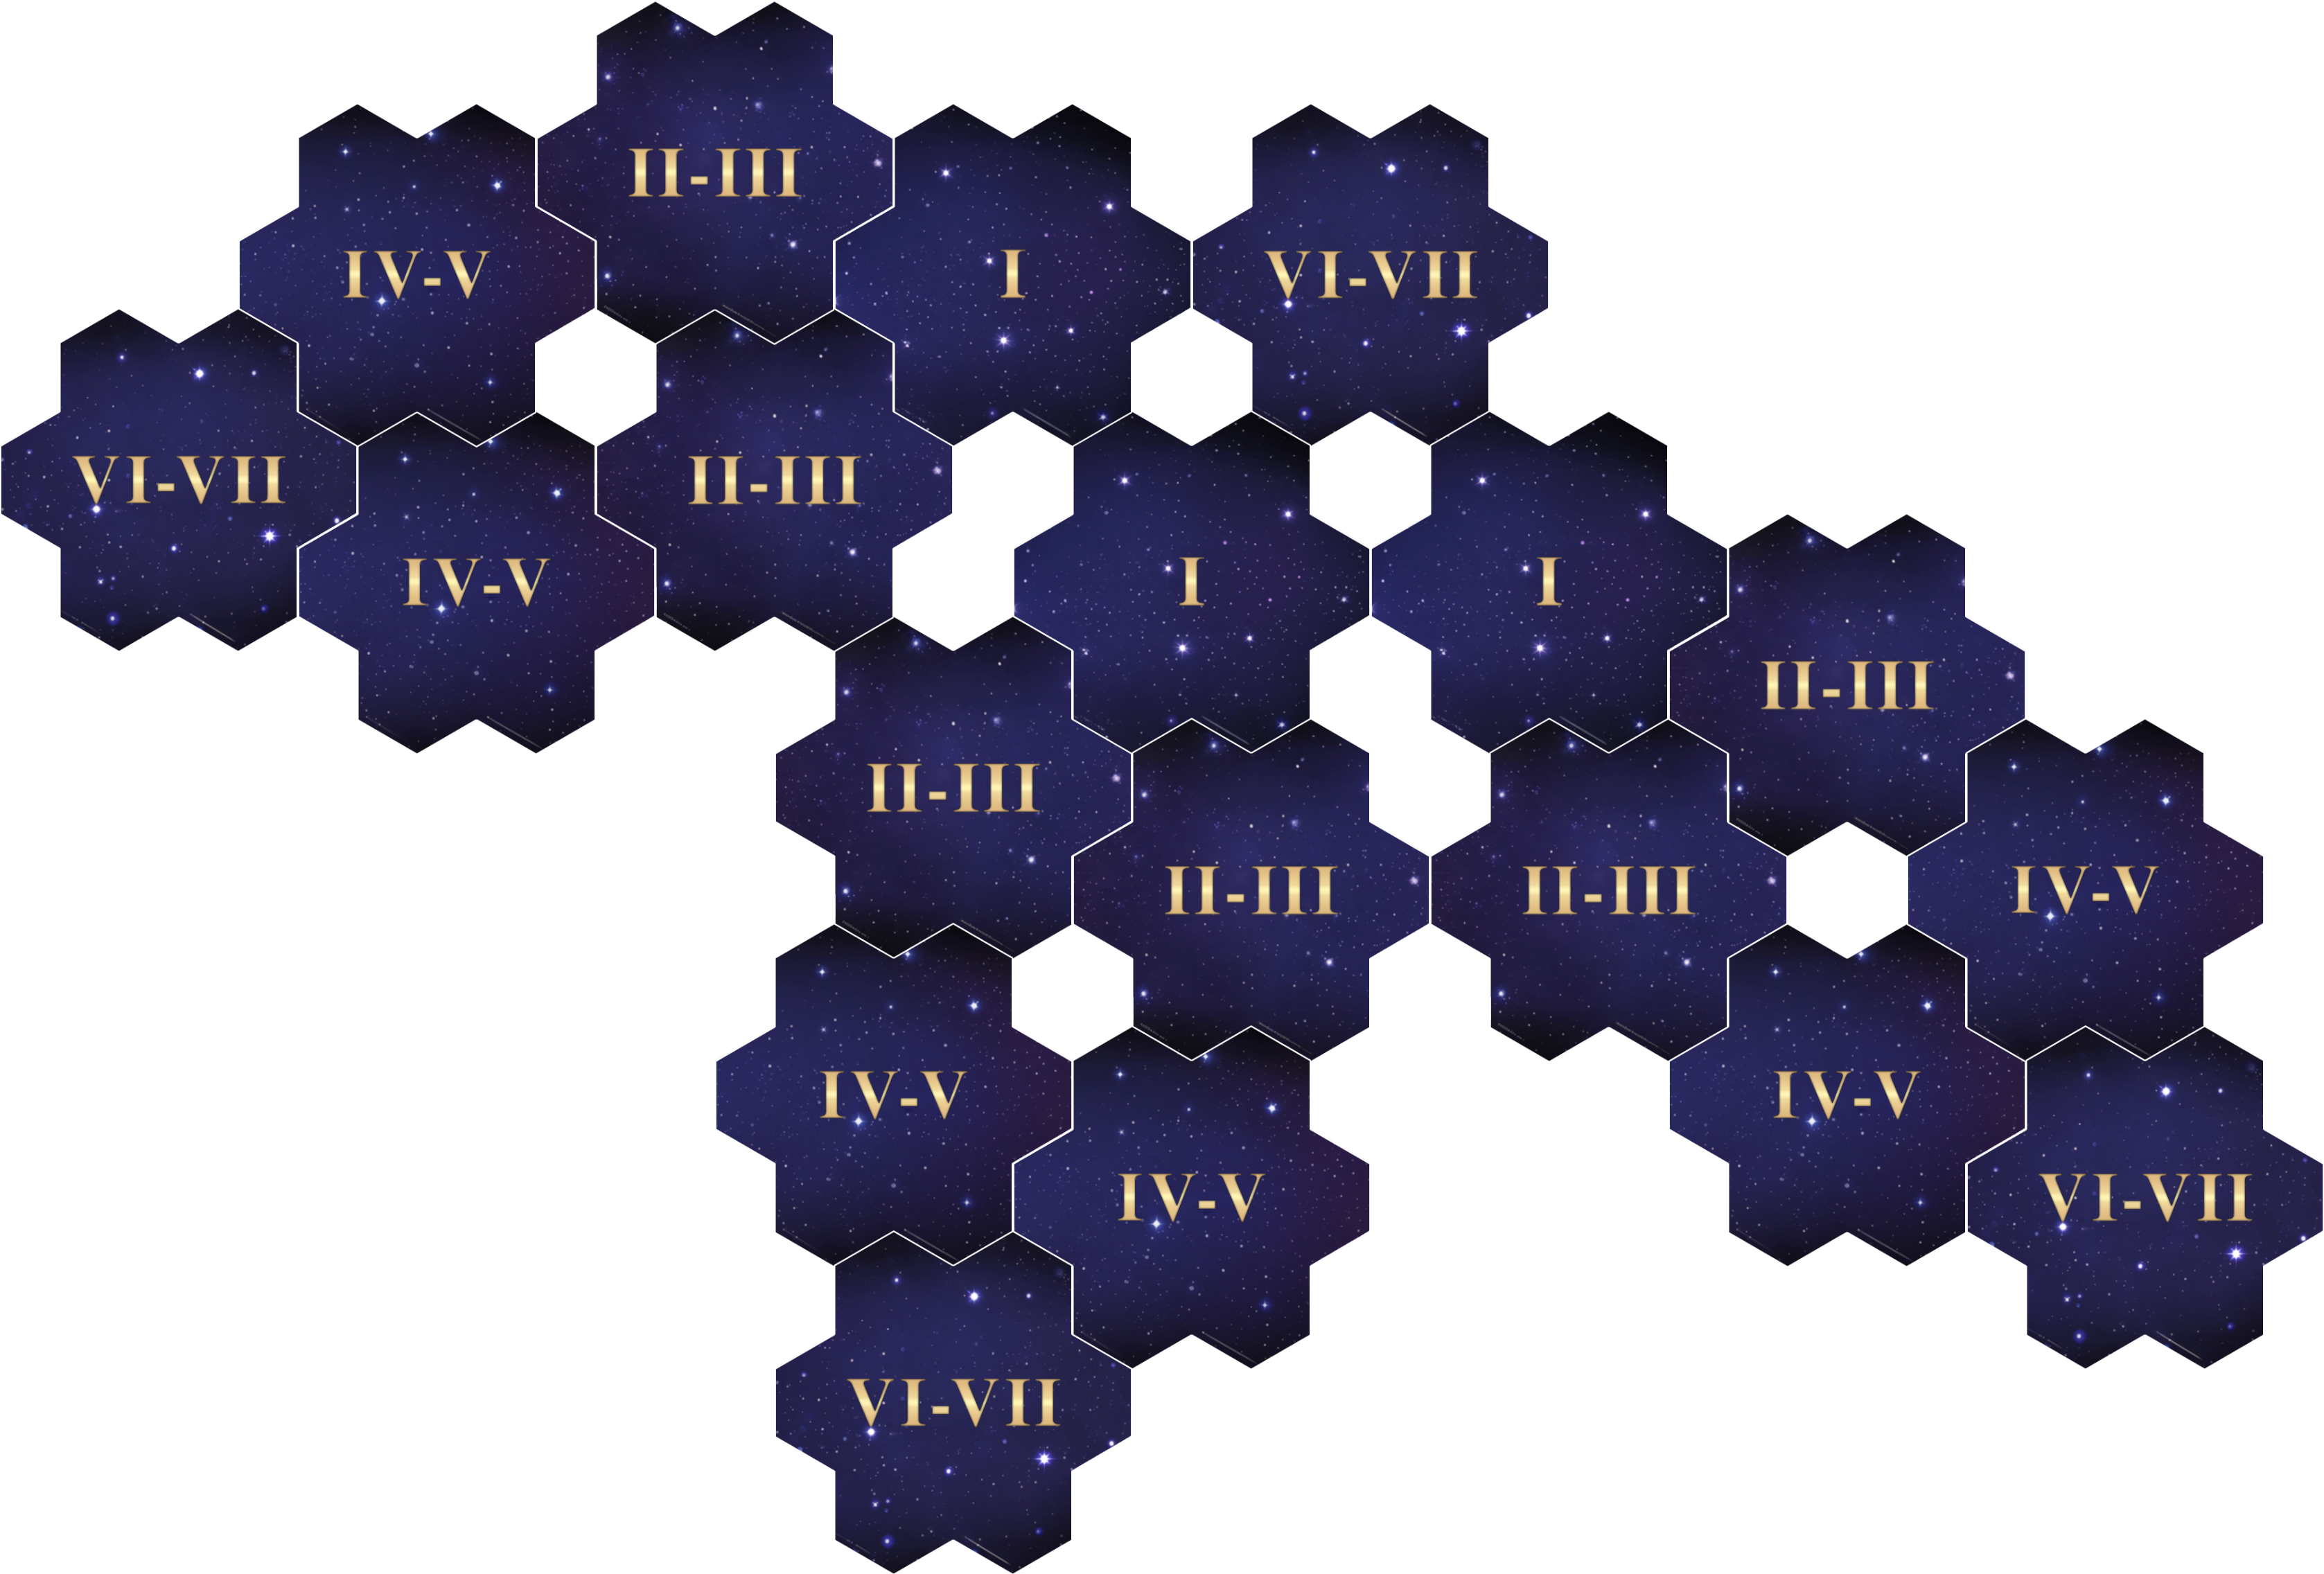
\includegraphics[width=0.38\paperwidth]{\maps/titans-3.png}
  \captionof{figure}{\textbf{3-PLAYER SCENARIO}}
\end{minipage}
\begin{minipage}{0.4\paperwidth}
  \centering
  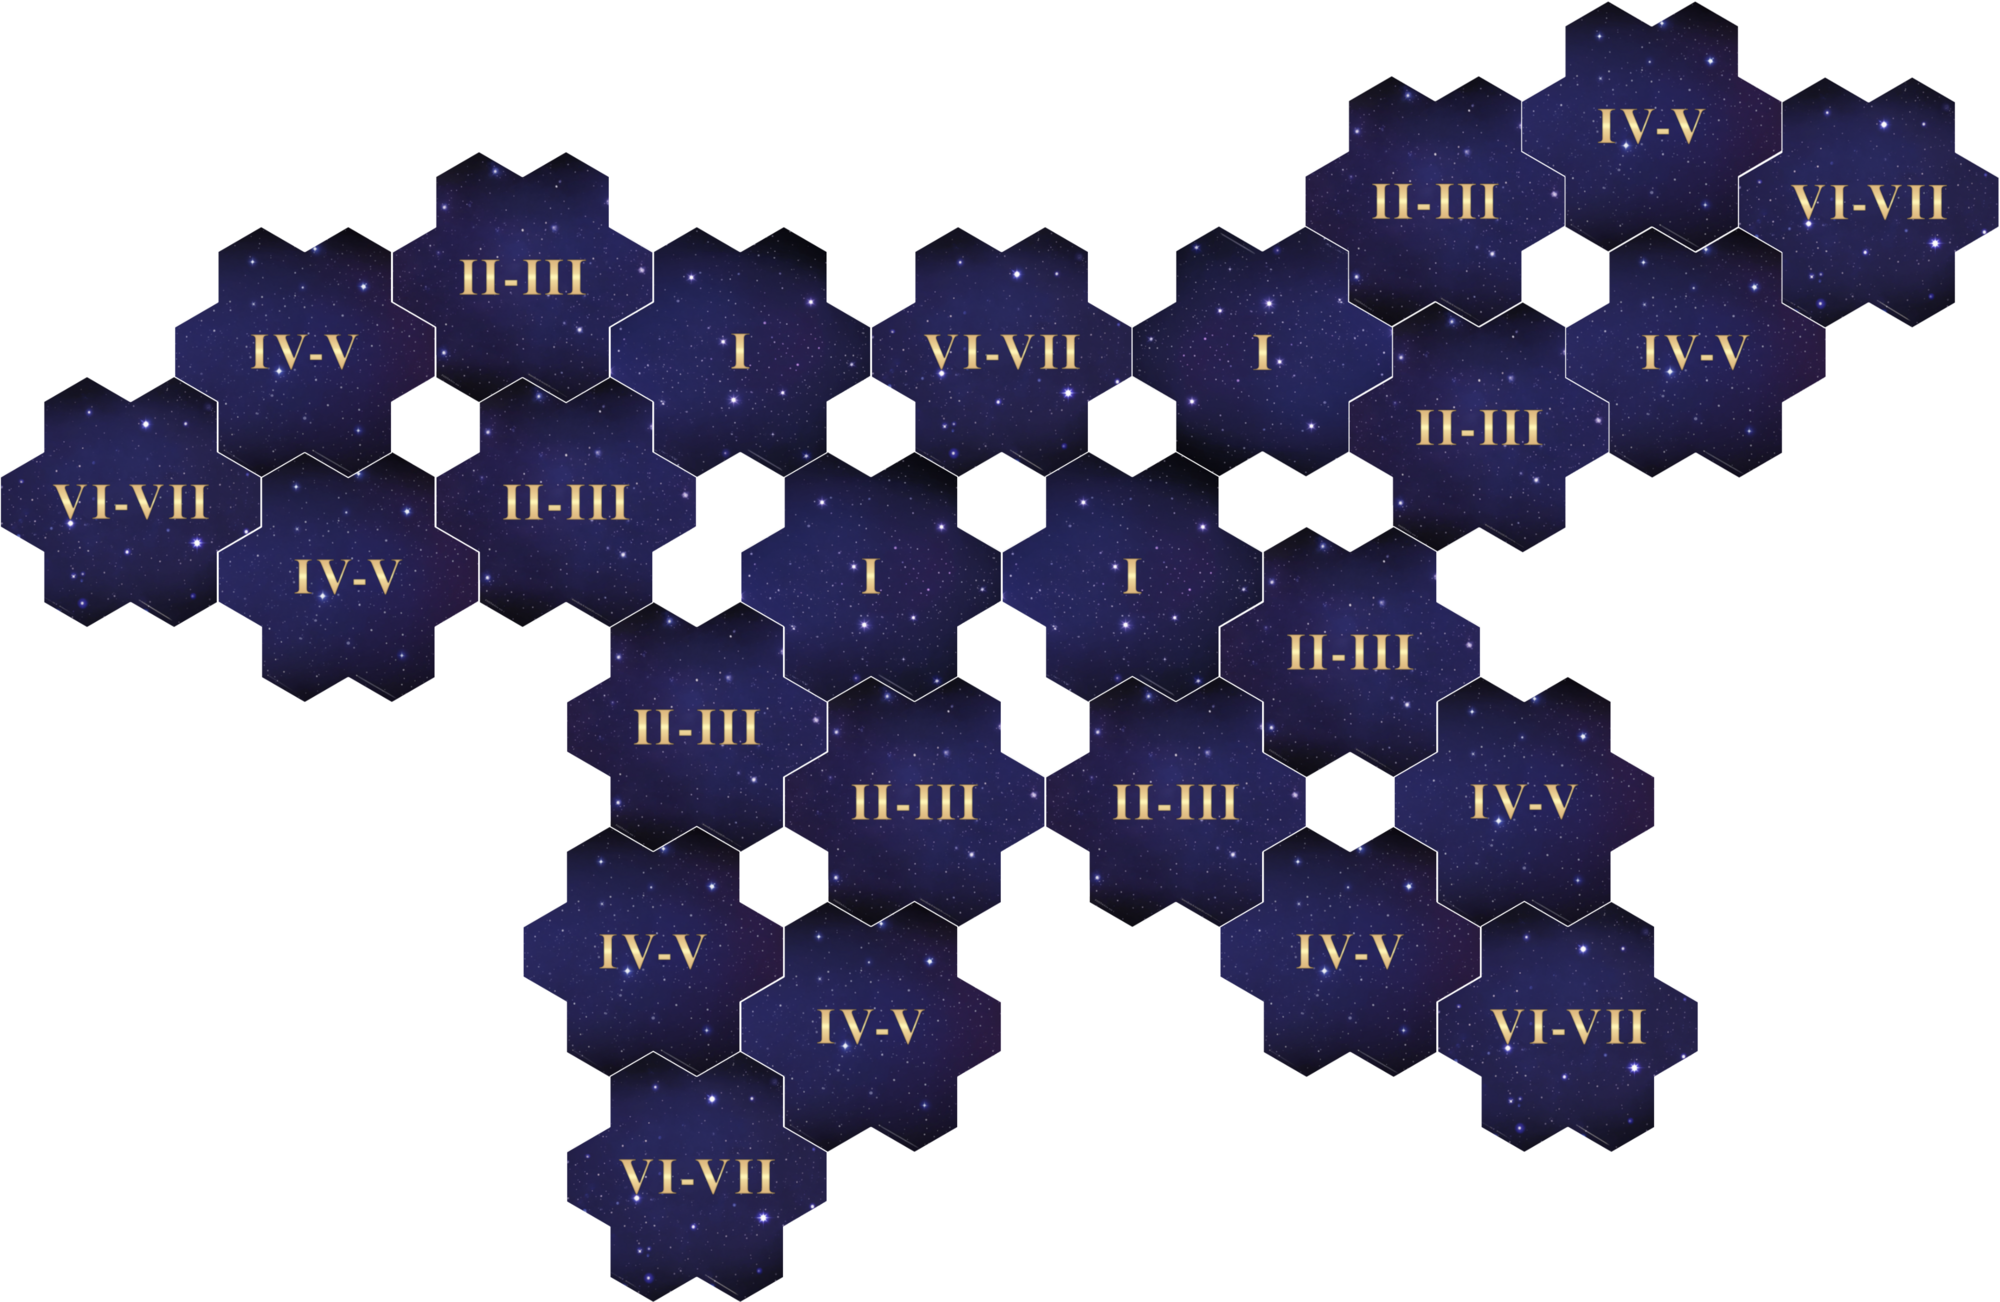
\includegraphics[width=0.38\paperwidth]{\maps/titans-4.png}
  \captionof{figure}{\textbf{4-PLAYER SCENARIO}}
\end{minipage}
\vspace{1em}
\linebreak
\begin{minipage}{0.4\paperwidth}
  \centering
  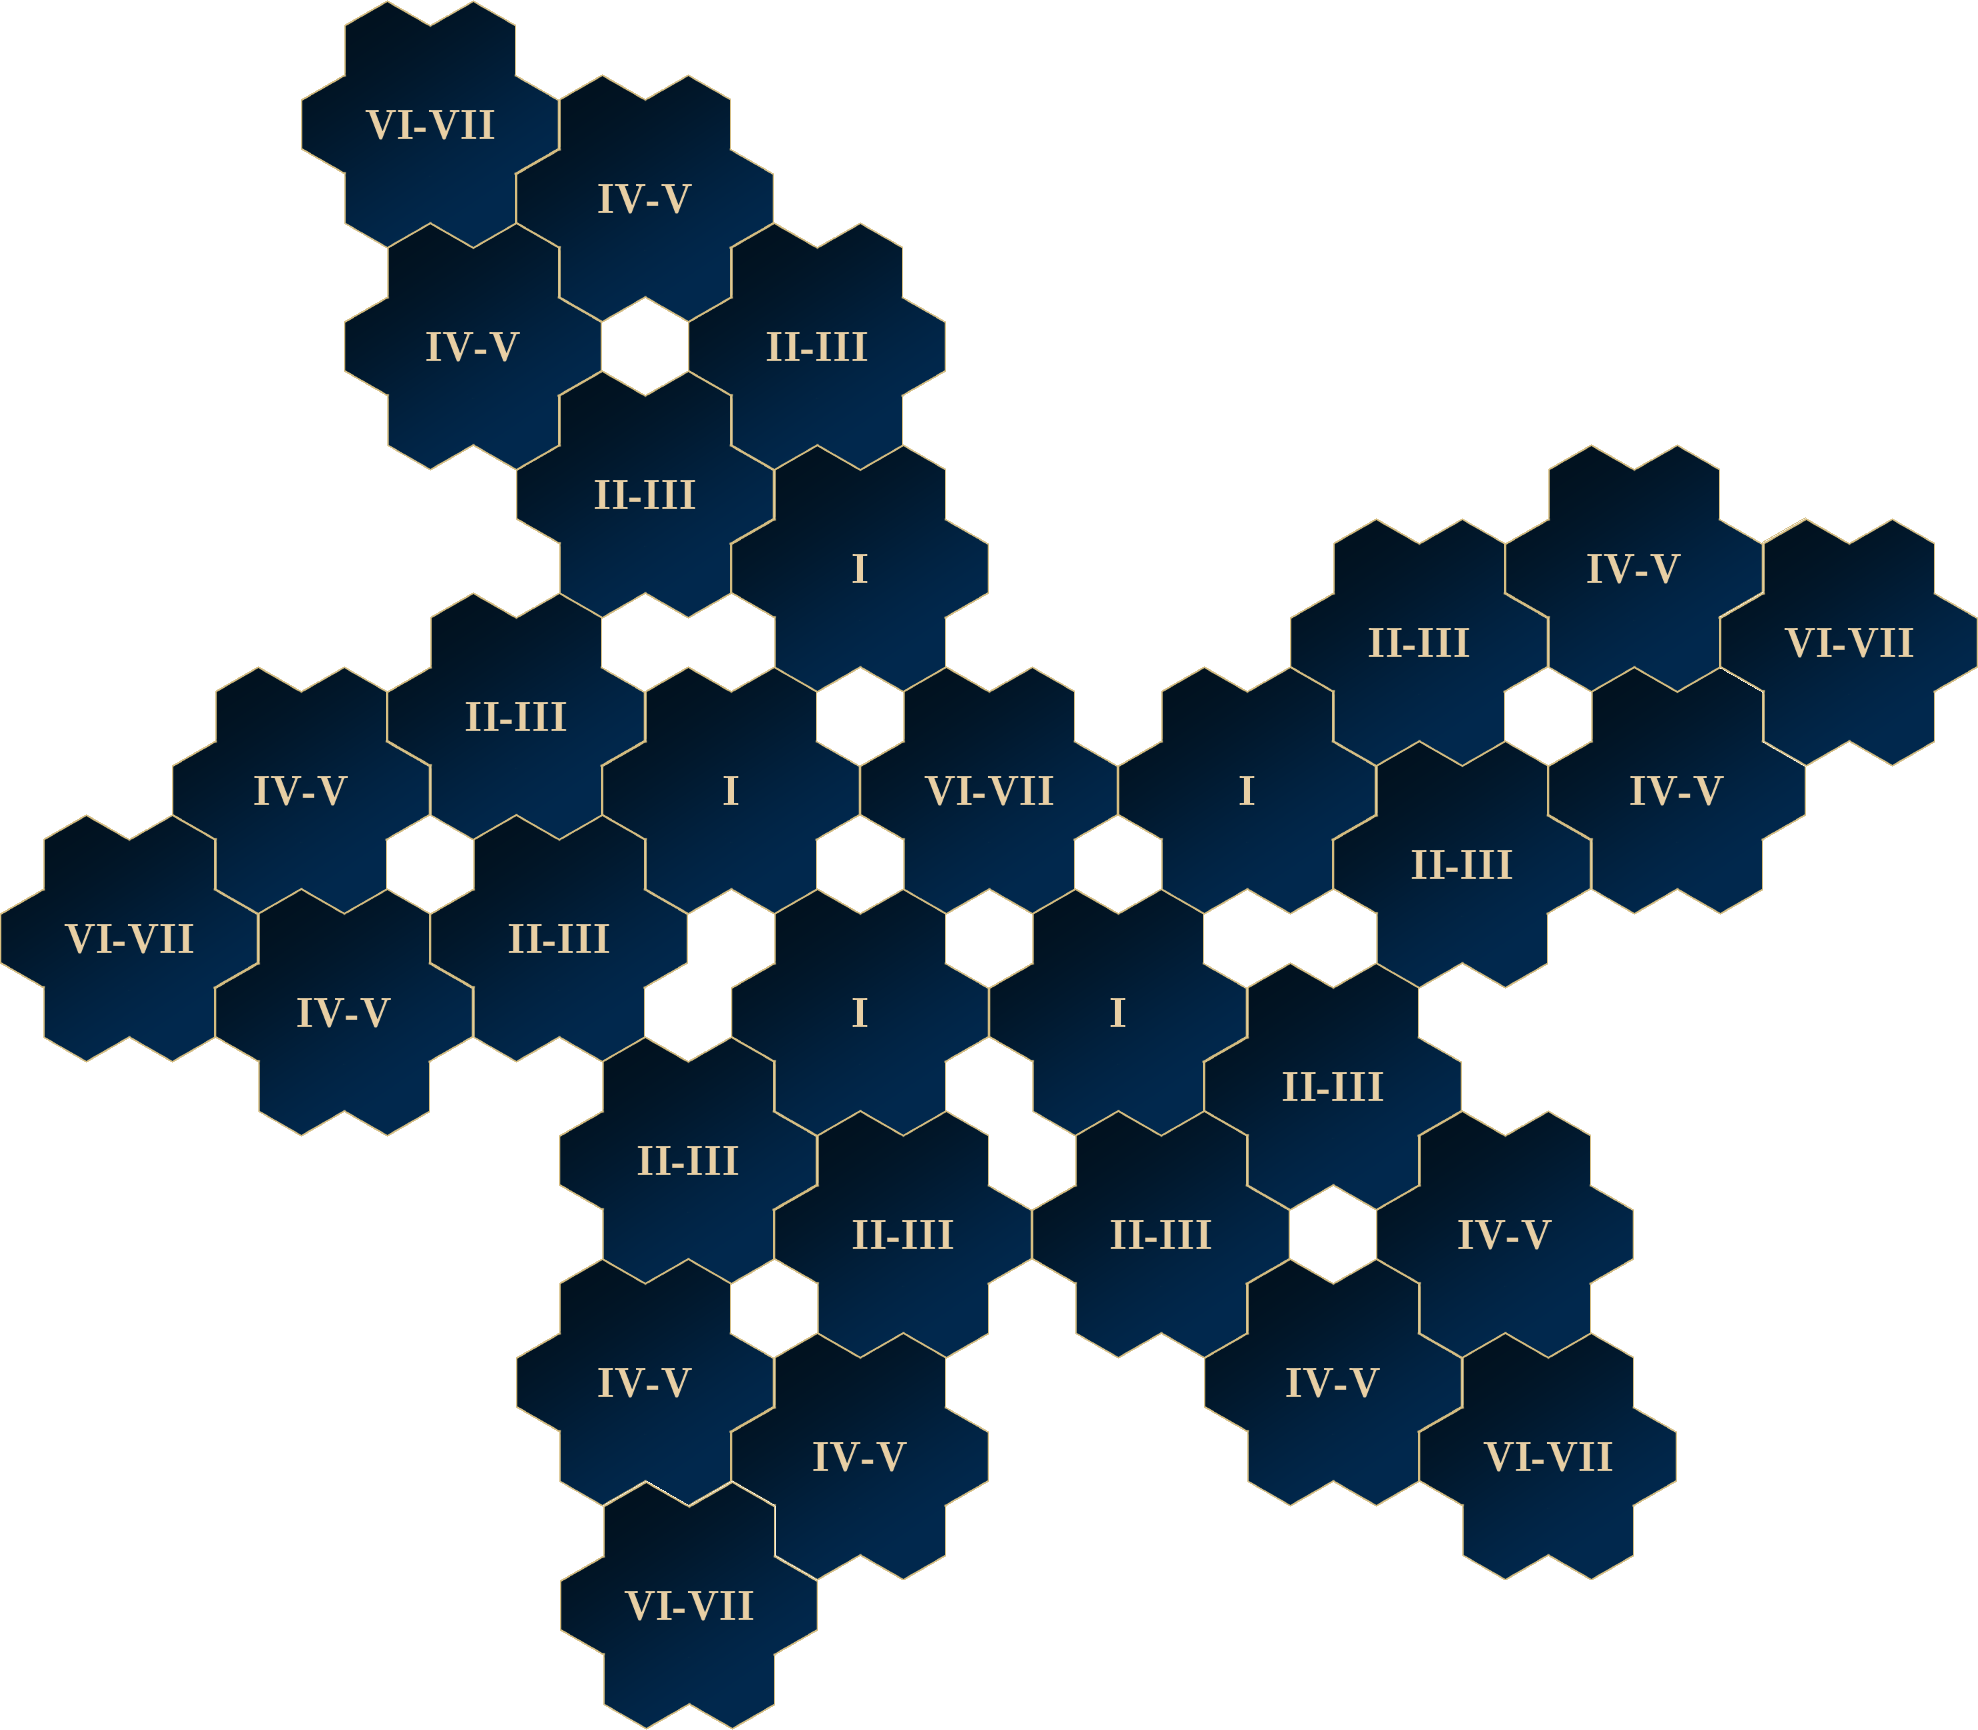
\includegraphics[width=0.38\paperwidth]{\maps/titans-5.png}
  \captionof{figure}{\textbf{5-PLAYER SCENARIO}}
\end{minipage}
\begin{minipage}{0.4\paperwidth}
  \centering
  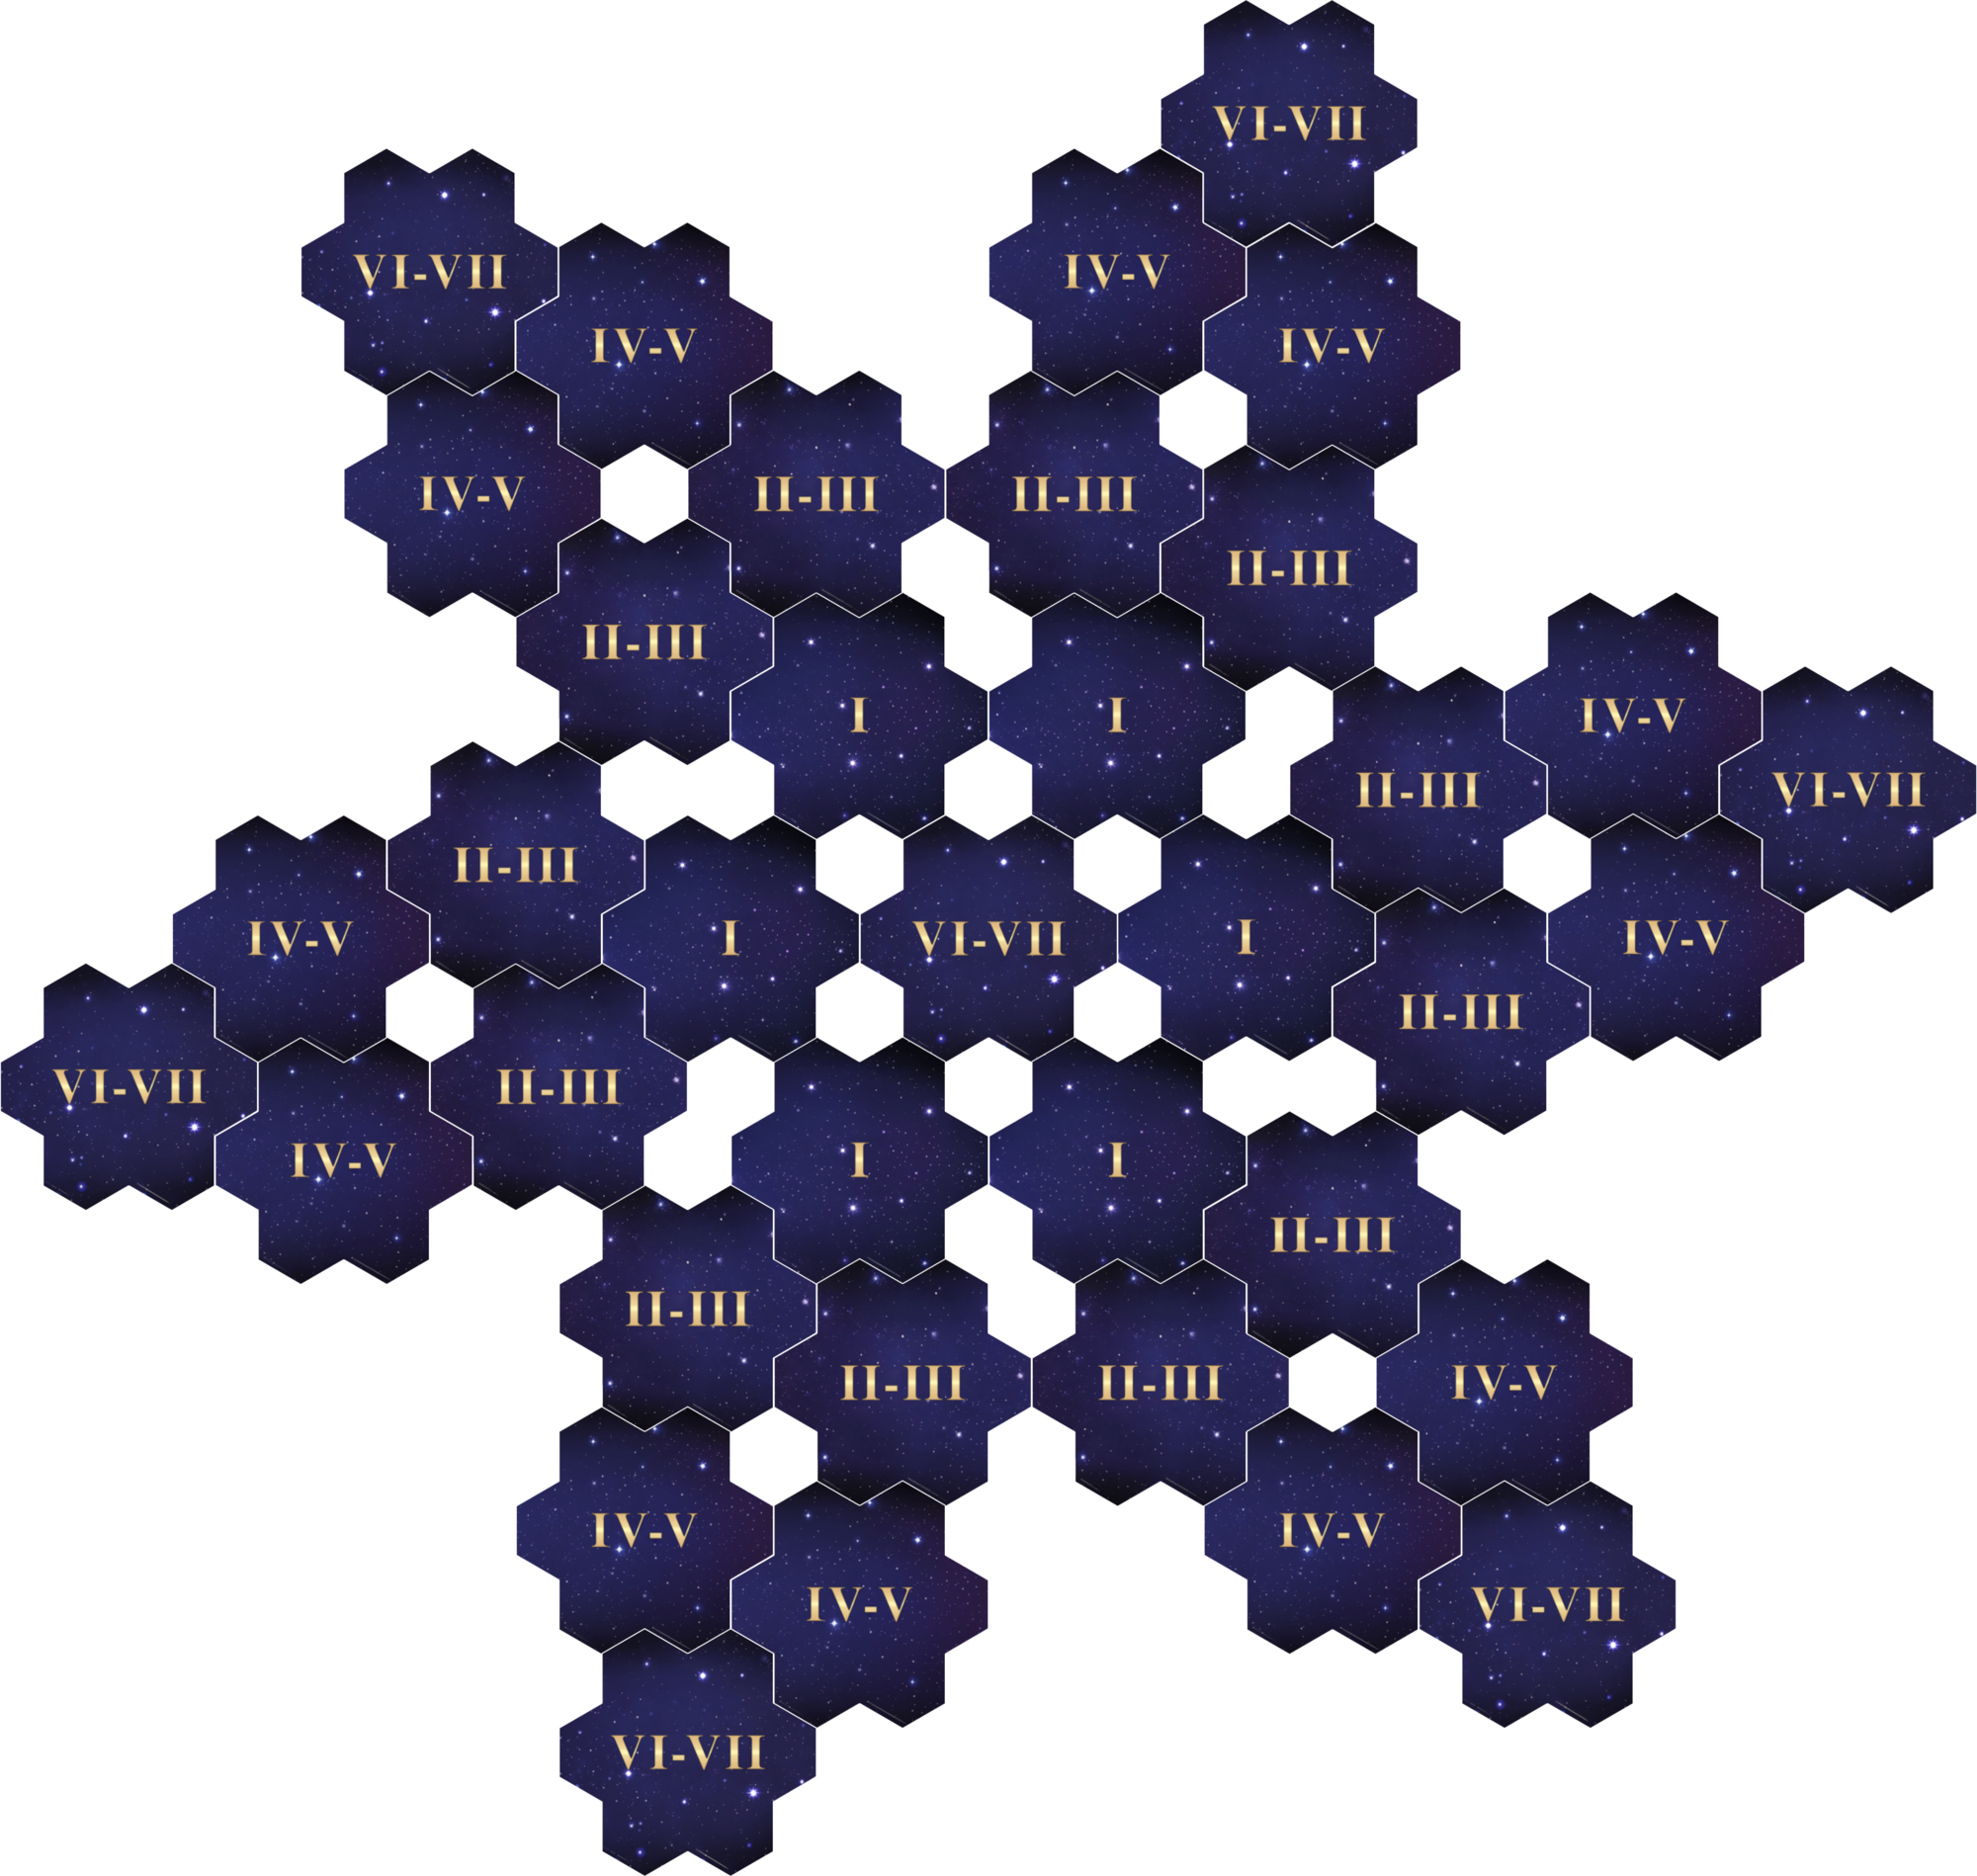
\includegraphics[width=0.38\paperwidth]{\maps/titans-6.png}
  \captionof{figure}{\textbf{6-PLAYER SCENARIO}}
\end{minipage}
